%
%  jif_paper1.tex
%
%  Created by Michael D. Schneider on 2015-04-27
%    <schneider@ucdavis.edu>
%
\documentclass[11pt, letterpaper]{article}

\usepackage[OT1]{fontenc}
\usepackage[in]{fullpage}

\usepackage[pdftex,pdfpagemode={UseOutlines},bookmarks,bookmarksopen,colorlinks,linkcolor={black},citecolor={black},urlcolor={red}]{hyperref}
\usepackage{graphicx}
\usepackage{bm}
\usepackage{amsmath,amssymb}
\usepackage{aas_macros}

\usepackage{mathptmx}  % times roman, including math (where possible)

\graphicspath{{figure/}}

%%%%%%%%%%%%%%%%%%%%%%%%%%%%%%%%%%%%%%%%%%%%%%%%%%%%%%%%%%%
% Macros
\newcommand{\half}{\frac{1}{2}}
\newcommand{\rhocrit}{\rho_{\rm crit}}
\newcommand{\rvir}{r_{\rm vir}}
\newcommand{\mvir}{m_{\rm vir}}
\newcommand{\om}{\Omega_{m}} 
\newcommand{\kv}{\mathbf{k}}
\newcommand{\xv}{\mathbf{x}}
\newcommand{\hmsun}{h^{-1}M_{\odot}}
\newcommand{\hmpc}{h^{-1}Mpc}
\newcommand{\hgpc}{h^{-1}{\rm Gpc}}
%%% Intrinsic galaxy properties (shape, size, flux, ...)
\newcommand{\galprops}{\omega}
%%% Point-spread function parameters for observing conditions
\newcommand{\psf}{{\Pi}}
%%% Observing conditions determining the PSF
\newcommand{\obscond}{\Omega}
%%% Pixel noise rms
\newcommand{\noiserms}{\sigma_{\rm pix}}
\newcommand{\noisermsni}{\sigma_{{\rm pix},n,i}}
%%% number of observed galaxies
\newcommand{\ngal}{n_{\rm gal}}
%%% number of observed epochs
\newcommand{\nepoch}{n_{\rm epoch}}
% PROBABILITY THEORY
\def\pr{{\rm Pr}}
\newcommand{\prf}[1]{\pr\left(#1\right)}
\def\data{{\mathbf{d}}}
\def\datamodel{\bar{\data}}
\def\datap{{\mathbf{d}^{\rm p}}}
\def\datai{\mathbf{d}_i}
\def\datapi{d^{\rm p}_i}
\newcommand{\trainingdata}{\mathbf{d}_{\rm train}}
%%%%%%%%%%%%%%%%%%%%%%%%%%%%%%%%%%%%%%%%%%%%%%%%%%%%%%%%%%%


%%%%%%%%%%%%%%%%%%%%%%%%%%%%%%%%%%%%%%%%%%%%%%%%%%%%%%%%%%%
%%%%%%%%%%%%%%%%%%%%%%%%%%%%%%%%%%%%%%%%%%%%%%%%%%%%%%%%%%%
\begin{document}
  
\title{Cosmic shear measurements from space and ground: \\Systematics from non-overlapping wavelengths}

\author{JIF collaborators}
%$^{1} Livermore National Laboratory, P.O. Box 808 L-210, Livermore, CA 94551-0808, USA.

\date{\today}

\maketitle
\tableofcontents

\begin{abstract}
	Galaxy morphologies can appear different at different wavelengths because distinct regions of 
	a galaxy can have different spectral energy distributions (SEDs). In this paper we demonstrate an 
	optimal algorithm to combine galaxy imaging data in different wavelength passbands to measure 
	the gravitational lensing distortions of galaxy shapes, or `cosmic shear.'
	We focus on the combination of space-based and ground-based imaging, which is
	further complicated by differing point-spread functions, pixel sizes, and detector characteristics.
	Assuming perfect knowledge of the SEDs of all components of a galaxy image, we show that a 
	full forward model of all joint imaging data improves shear inferences by a factor of XXX. 
	Assuming instead only weak prior information on galaxy SED components, the shear inference from 
	combined imaging from the Large Synoptic Survey Telescope (LSST) and WFIRST-AFTA would be improved 
	by a factor of YYY if WFIRST-AFTA contained an optical passband overlapping those of LSST.
\end{abstract}

% -----------------------------------------------------------------------------
\section{Introduction} % (fold)
\label{sec:introduction}

% section introduction (end)


% -----------------------------------------------------------------------------
\section{Joint image modeling framework} % (fold)
\label{sec:joint_image_modeling_framework}
{\it TODO: Describe how JIF works here, including the statistical framework and 
computing implementations.}

We are interested in the posterior probability distribution for the properties of a galaxy
$\galprops_{n}$ (e.g., size, flux, ellipticity) given some imaging data pixel values
$\datai$ in multiple epochs $i$. By marginalizing over uncertainties in the PSF model, 
which can be partially degenerate with galaxy properties, the posterior can be 
factored as,
\begin{equation}
	\prf{\galprops_{n} | \left\{\datai, \noisermsni, \obscond_{i}\right\}_{i=1}^{\nepoch}, 
		\trainingdata} \propto
	\prod_{i=1}^{\nepoch}
	\left[	
	\int d\psf_{ni}\,
	\prf{\datai | \galprops_n, \noisermsni, \psf_{ni}}\,
	\prf{\psf_{ni} | \obscond_{i}}
	\right]
	\prf{\galprops_{n}| \trainingdata},
\end{equation}
where the PSF in epoch $i$ at the location of galaxy $n$ is $\psf_{ni}$,
$\obscond_{i}$ indicates any knowledge about the observing conditions that affect 
the PSF in epoch $i$ (such as atmosphere seeing or temperature of the telescope), 
$\noisermsni$ denotes the pixel noise rms (or other noise model parameter) in the 
vicinity of galaxy $n$ in epoch $i$, and $\trainingdata$ is any external data that is 
used to train the model for the distribution of galaxy properties.

\begin{figure}[htb]
	\centerline{
		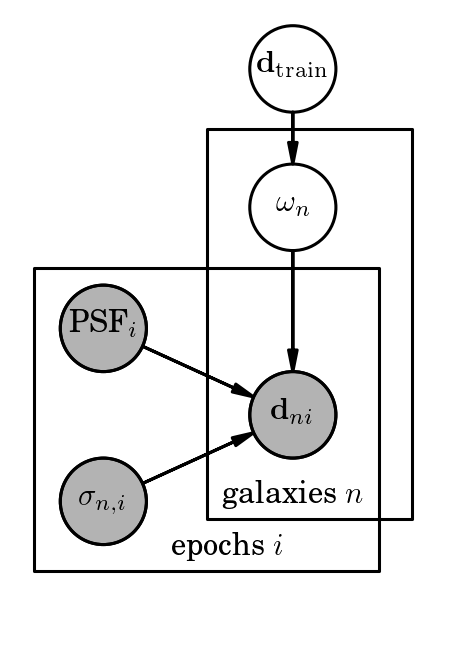
\includegraphics[width=0.5\textwidth]{pgm.png}
	}
	\caption{\label{fig:pgm}Probabilistic graphical model for our joint model of 
	galaxy images in multiple observation epochs (where the designation 
	`epoch' include observations with different telescopes).}
\end{figure}

% -------------------------------------
\subsection{Galaxy image models} % (fold)
\label{sub:galaxy_image_models}
{\it Galsim wrapper}
% subsection galaxy_image_models (end)

% -------------------------------------
\subsection{The probability distribution of galaxy model parameters} % (fold)
\label{sub:the_probability_distribution_of_galaxy_model_parameters}
{\it From space-base imaging...}
% subsection the_probability_distribution_of_galaxy_model_parameters (end)

% -------------------------------------
\subsection{Noise models} % (fold)
\label{sub:noise_models}

% subsection noise_models (end)

% -------------------------------------
\subsection{Monte Carlo sampling} % (fold)
\label{sub:monte_carlo_sampling}

% subsection monte_carlo_sampling (end)

% section joint_image_modeling_framework (end)


% -----------------------------------------------------------------------------
\section{Results: combining space and ground imaging data} % (fold)
\label{sec:results_combining_space_and_ground_imaging_data}

% section results_combining_space_and_ground_imaging_data (end)


% -----------------------------------------------------------------------------
\section{Conclusions} % (fold)
\label{sec:conclusions}

% section conclusions (end)

\end{document}

